%%%%%%%%%%%%%%%%%%%%%%%%%%%%%%%%%%%%%%%%%%%%%%%%%%%%%%%%%%%%%%%%%%%%%%%%%%%%%
%% Descr:       Vorlage für Berichte der DHBW-Karlsruhe, Ein Kapitel
%% Author:      Prof. Dr. Jürgen Vollmer, vollmer@dhbw-karlsruhe.de
%% $Id: kapitel2.tex,v 1.5 2017/10/06 14:02:51 vollmer Exp $
%%  -*- coding: utf-8 -*-
%%%%%%%%%%%%%%%%%%%%%%%%%%%%%%%%%%%%%%%%%%%%%%%%%%%%%%%%%%%%%%%%%%%%%%%%%%%%%%%

\section{OpenGL}
\label{chap:OpenGL}
\subsection{Projektionen}
\subsection{Shader}

\section{Softwarearchitektur}
\label{chap:Softwarearchitektur}
Komponenten in Form von Klassen, Objekten oder Bibliotheken und deren Verbindungen zwischen einzelnen Komponenten beschreibt die Architektur 
eines Softwaresystems. Vielmehr geht es bei der Software-Architektur darum, Anforderungen und deren Zusammenhänge untereinander von dem zu 
konstruierenden System zu beschreiben und nicht einen detaillierten Entwurf vorzulegen. Jedoch hat die Architektur einen enormen Einfluss 
auf die qualitativen und nicht-funktionalen Eigenschaften des daraus resultierenden Systems. 
\\ 
\linebreak
Die Terminologie nach dem \textit{IEEE-Standard 1471-2000} zur Software Architekturbeschreibung, deren Aufgaben und Zweck \cite{swarchitekturieee.2005} 
sind wie folgt definiert: 
\begin{quote}
    Die grundlegende Organisation eines Systems, dargestellt durch dessen Komponenten, deren Beziehungen zueinander und zur Umgebung sowie den 
    Prinzipien, die den Entwurf und die Evolution des Systems bestimmen. \cite{architektursw.2006f}
\end{quote}
Softwarearchitektur bietet viele Möglichkeiten ein System zu entwerfen und Anforderungen und Eigenschaften umzusetzen, daher gibt es auch 
hier viele Ansätze, Lösungen und Abwandlungen, um den Standards und Richtlinien gerecht zu werden. Beispiele dafür sind unter anderem die 
Modulare Software Architektur (\ref{chap:Modulare Software Architektur}) und das Architektur-Entwurfsmuster MVVM (\ref{chap:MVVM}).
\\
Das Buch \textit{Design Patterns - Elements of Reusable Object-Oriented Software} von E. Gamma, R. Helm, R. Johnson und J. Vlissides befasst 
sich mit den verschiedensten Möglichkeiten und Ausprägungen der Softwarearchitektur. 
\\ 
Im Rahmen dieser Ausarbeitung findet keine Aufzählung und Beschreibung verschiedener Arten der Architekturmuster und -stile statt, lediglich die 
für das Projekt verwendeten Muster werden in folgenden Kapiteln aufgegriffen. 
\\ 
\linebreak
Die Abbildung \ref{pic:mvcdiagram} veranschaulicht eine vereinfachte Struktur eines Architekturmusters und deren Komponenten und Zusammenhänge 
zueinander. Die Zeichnung dient zur Veranschaulichung, um darzulegen wie ein Architekturdiagramm aussehen kann, bzw. wie die allgemeine 
Struktur repräsentiert wird.
\begin{figure}[hbt!]
    \centering
    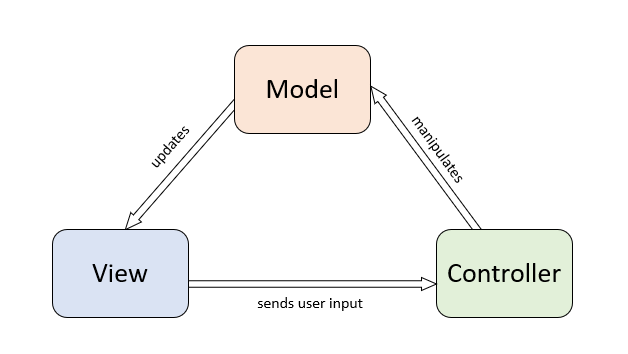
\includegraphics[width=15cm,height=7.5cm,keepaspectratio]{2GrundlagenX/Bilder/MVCArchitecture.png}
    \caption{MVC Architektur Diagramm \cite{mvcbild.2020}}
    \label{pic:mvcdiagram}
\end{figure} 
Im Falle dieser Abbildung wurde das Strukturmuster \ac{MVC} ausgewählt, welches die zu sehenden Komponenten in drei in sich 
geschlossene und unabhängige Fragmente unterteilt die miteinander interagieren. 
\\ 
\linebreak
Neben der Strukturierung von Systemen und Applikationen kann die Modellierung einer Softwarearchitektur auch dabei helfen eine Architektur genauer 
zu beschreiben und zu dokumentieren. Ebenso können Diagramme auch das Management sowie die Planung beeinflussen und verstärken. Die Modellierung 
der Softwarearchitektur stellt somit keinen Selbstzweck dar, sondern bietet einen Mehrwert indem es zur Verständigung, Dokumentation und 
Kommunikation zwischen Entwicklern und Kunden zusätzlich beiträgt. 
\\ 
Durch die Modellierung der Architektur kann frühzeitig eine sinnvolle Evaluierung und Bewertung des Entwurfs durchgeführt werden. Mit diesen 
entstehenden Bewertungen können folgende Schritte besser geplant und umgesetzt werden. 
\\ 
\linebreak
Eine weitere Variante, bzw. Ausprägung der Software-Architektur ist die Modulare Software Architektur (siehe Abschnitt \ref{chap:Modulare Software Architektur}).
\subsection{Modulare Software Architektur}
\label{chap:Modulare Software Architektur}
\subsection{MVVM}
\label{chap:MVVM}
\subsection{Android Architecture Components}
\label{chap:AAC}



\section{Datenmodellierung}
\label{chap:Datenmodellierung}